\documentclass[UTF8,AutoFakeBold,AutoFakeSlant,zihao=-4]{ctexart}
\usepackage[a4paper,left=2.4cm,right=2.4cm,top=2.6cm,bottom=2.38cm,includeheadfoot]{geometry}   % 设置页面大小
\usepackage{fontspec} % 字体
\usepackage{setspace} % 设置行距
\usepackage{graphicx} % 图片
\usepackage{fancyhdr} % 页眉页脚
\usepackage{pdfpages} % 插入 PDF
\usepackage{setspace} % 设置行距
\usepackage{booktabs} % 表格
\usepackage{multirow} % 表格
\usepackage{caption} % 图片和表格的 caption
\usepackage{subcaption} 
\usepackage{float} 


\newcommand{\coursename}{《Python程序设计》}
\newcommand{\coursenumber}{U08M11077.01}
\newcommand{\proname}{2048小游戏开发}
\newcommand{\members}{敖冠舒~唐中磊~王骏松~王一帆}
\newcommand{\phone}{134~0324~7575}
\newcommand{\protime}{2022年12月}

% 定义 caption 字体为楷体
\DeclareCaptionFont{kaiticaption}{\kaishu \normalsize}

% 设置图片的 caption 格式
\renewcommand{\thefigure}{\thesection-\arabic{figure}}
\captionsetup[figure]{font=small,labelsep=space,skip=10bp,labelfont=bf,font=kaiticaption}

% 设置表格的 caption 格式
\renewcommand{\thetable}{\thesection-\arabic{table}}
\captionsetup[table]{font=small,labelsep=space,skip=10bp,labelfont=bf,font=kaiticaption}

% 定义一个概念
\newtheorem{definition}{概念}[section]

% 输出大写数字日期
\CTEXoptions[today=big]


\setromanfont{Times New Roman}



% 设置文档标题深度
\setcounter{tocdepth}{3}
\setcounter{secnumdepth}{3}

%%
% 设置一级标题、二级标题格式
% 一级标题:小三,宋体,加粗,段前段后各半行
\ctexset{section={
  format={\raggedright \bfseries \songti \zihao{-3}},
  beforeskip = 24bp plus 1ex minus .2ex,
  afterskip = 24bp plus .2ex,
  fixskip = true,
  name = {,.}
  }
}
% 二级标题:小四,宋体,加粗,段前段后各半行
\ctexset{subsection={
  format = {\bfseries \songti \raggedright \zihao{4}},
  beforeskip =24bp plus 1ex minus .2ex,
  afterskip = 24bp plus .2ex,
  fixskip = true,
  }
}

%%
% 文档开始
\begin{document}

% 报告封面
\topskip=0pt

\begin{titlepage}
  \vspace*{20mm}
  \centering
  \hspace{0mm}\heiti\fontsize{30pt}{30pt}\selectfont{西北工业大学}

  \vspace{13mm}

  \hspace{0mm}\heiti\fontsize{20pt}{20pt}\selectfont{课程设计(大作业)报告}

  \vspace{40mm}

  \flushleft
  \begin{spacing}{2.2}


    \hspace{36mm}\songti\fontsize{16pt}{16pt}\selectfont{\textbf{课程名称:}\underline{\makebox[72mm][c]{\coursename}}}

    \hspace{36mm}\songti\fontsize{16pt}{16pt}\selectfont{\textbf{课程编号:}\underline{\makebox[72mm][c]{\coursenumber}}}

    \hspace{36mm}\songti\fontsize{16pt}{16pt}\selectfont{\textbf{设计题目:}\underline{\makebox[72mm][c]{\proname}}}

    \hspace{36mm}\songti\fontsize{16pt}{16pt}\selectfont{\textbf{组员名单:}\underline{\makebox[72mm][c]{\members}}}

    \hspace{36mm}\songti\fontsize{16pt}{16pt}\selectfont{\textbf{联系方式:}\underline{\makebox[72mm][c]{\phone}}}

    \hspace{36mm}\songti\fontsize{16pt}{16pt}\selectfont{\textbf{设计时间:}\underline{\makebox[72mm][c]{\protime}}}
  \end{spacing}

  \vspace{47mm}


\end{titlepage}



%%插入一页目录
\newpage
\tableofcontents


% 正文开始
\pagestyle{fancy}
% 正文从第一页开始计算页码
\setcounter{page}{1}
% 页眉和页脚(页码)的格式设定
\fancyhf{}
\fancyhead[R]{\fontsize{10.5pt}{10.5pt}\selectfont{西北工业大学课程设计(大作业)报告}}
\fancyfoot[R]{\fontsize{9pt}{9pt}\selectfont{\thepage}}
\renewcommand{\headrulewidth}{1pt}
\renewcommand{\footrulewidth}{0pt}

% 正文 22 磅的行距,段前段后间距为 0
\setlength{\parskip}{0em}
\renewcommand{\baselinestretch}{1.53}
% 正文首行悬挂 1.02cm
\setlength{\parindent}{1.02cm}

% 内容开始
\section{设计概述}
\subsection{设计目的}
本项目通过Python语言实现2048小游戏,从而掌握《Python程序设计》课程中的知识,更好地掌握Python语言的基本语法和编程思想,提高编程能力。与此同时,本项目还可以让我们更好地了解游戏开发的基本流程,从而更好地掌握游戏开发的基本知识,在此过程中队员分工合作,提高团队协作能力。


\subsection{设计内容}
本项目通过Python语言实现2048小游戏,实现游戏的基本功能,包括游戏界面的显示、游戏的开始、游戏的暂停、游戏的结束、游戏的重新开始、游戏的分数统计等功能。除此之外,还实现了游戏的难度选择、AI模式的实现等高级功能,通过AI模式,可以让玩家在游戏中获得更好的游戏体验。

\subsection{应用平台}
\begin{table}[H]
  \centering
  \caption{硬件、软件环境一览表}
  \label{tab:soft-hardware}
  \begin{tabular}{@{}lcl@{}}
    \toprule
                              & 指标     & \multicolumn{1}{c}{版本参数} \\ \midrule
    \multirow{2}{*}{硬件环境} & CPU      & AMD R7-5800H               \\ \cmidrule(l){2-3}
                              & RAM      & 16 GB                         \\ \midrule
    \multirow{2}{*}{软件环境} & 操作系统 & Windows 11 Pro 22H2 \\ \cmidrule(l){2-3}
                              & Python   & Python 3.8.15                 \\ \bottomrule
  \end{tabular}
\end{table}



\subsection{开发工具}
\begin{table}[H]
  \centering
  \caption{开发工具一览表}
  \label{tab:dev-tool}
  \begin{tabular}{@{}lcl@{}}
    \toprule
    工具 & 版本 & 用途 \\ \midrule
    PyCharm & 2022.3 & 代码编写 \\ 
    Anaconda & 2022.11.1 & Python环境管理 \\ \bottomrule
  \end{tabular}
\end{table}



\subsection{软件库}
\begin{table}[H]
  \centering
  \caption{软件库一览表}
  \label{tab:soft-lib}
  \begin{tabular}{@{}lcl@{}}
    \toprule
    库名 & 版本 & 用途 \\ \midrule
    pygame & 2.1.2 & 游戏界面的显示 \\ 
    numpy & 1.24.0 & 数组的处理 \\
    \bottomrule
  \end{tabular}
\end{table}




\subsection{软件测试}
本程序的测试数据主要包括游戏界面的显示、游戏的开始、游戏的暂停、游戏的结束、游戏的重新开始、游戏的分数统计等功能的测试,以及游戏的难度选择、自动托管模式的实现等高级功能的测试。其中,游戏界面的显示、游戏的开始、游戏的暂停、游戏的结束、游戏的重新开始、游戏的分数统计等功能的测试,主要通过人工测试的方式进行测试,而游戏的难度选择、自动托管模式的实现等高级功能的测试,主要通过自动化测试的方式进行测试。
%另起一页
\clearpage

\section{详细设计}
\subsection{总体方案}
本项目采用模块化和面向对象的方法,将程序分为多个类,每个类负责一个功能,类与类之间通过接口进行通信,类与类之间的通信方式采用函数调用的方式,类与类之间的数据传递采用参数传递的方式,类与类之间的数据共享采用全局变量的方式。

具体来说,本项目采用的类有:Main主函数类、按钮类、Ai类等,用于实现游戏界面的显示、开始、暂停、结束、重新开始、分数统计等功能。

本项目使用四个.py文件实现上述功能,分别是main.py、config.py、ai.py和game.py,其中main.py是主函数,用于调度各个模块以实现功能;config.py是配置文件,主要负责游戏参数的设置;ai.py是AI算法文件,用于实现游戏的AI模式,game.py是游戏文件,用于绘制游戏界面,实现具体的游戏功能。

\subsection{功能实现}
此部分要分析任务书,并给出初步方案,要体现出复杂系统的概念,约写 2 至 3 页。

\subsubsection{XXX功能的实现}
(详细描述功能实现的原理和方法。)
(并简要描述你的程序中各函数程序代码的实现(如算法、数据结构),不要大段的贴代码)

\subsubsection{XXX功能的实现}
(详细描述功能实现的原理和方法。)
(并简要描述你的程序中各函数程序代码的实现(如算法、数据结构),不要大段的贴代码)

\begin{figure}[!ht]
  \centering
  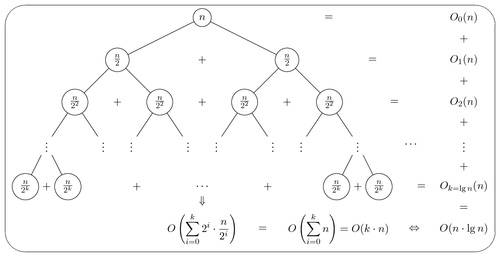
\includegraphics[width=0.6\linewidth]{img/merge-sort-recursion-tree}
  \caption{Merge sort recursion tree:一张示意图}
  \label{fig:mergesort}
\end{figure}



\section{完成情况}

\subsection{程序运行结果}
(程序运行的中间和最后的结果,并配上说明

\subsection{程序使用说明}
(程序的使用说明,包括程序的运行环境、运行方法、运行结果等)

\subsection{主要研究过程}
(详细描述你设计、调试程序的过程,类似开发日记)

\section{设计总结}

\subsection{成员分工}
(详细描述每位成员姓名、学号、班级、院系,以及分工完成的任务)

\subsection{存在的问题}
(描述你的程序存在的问题,以及你的改进意见)

\subsection{改进措施}
(对你设计的程序,未来可以从哪些具体地方使用什么措施进行改进)

\subsection{课程收获}
(对每位成员参加本课程的感想和收获)

\subsection{对课程的建议}

\section{附录}
\subsection{程序源代码}
见电子压缩文档XXX.zip文件
(无需粘贴程序源码)

\subsection{其他}
若有其他附录文件,可写于此处,组织好格式

\begin{table}[!ht]
  \centering
  \caption{硬件、软件环境}
  \label{tab:soft-hardware}
  \begin{tabular}{@{}lcl@{}}
    \toprule
                              & 指标     & \multicolumn{1}{c}{版本参数} \\ \midrule
    \multirow{2}{*}{硬件环境} & CPU      & Intel i7-6500U               \\ \cmidrule(l){2-3}
                              & RAM      & 8 GB                         \\ \midrule
    \multirow{2}{*}{软件环境} & 操作系统 & \begin{tabular}[c]{@{}l@{}}Windows 10 Pro x86\_64\\  Ubuntu 18.04.3 LTS\end{tabular}    \\ \cmidrule(l){2-3}
                              & Python   & Python 3.7.6                 \\ \bottomrule
  \end{tabular}
\end{table}



\begin{table}[!ht]
  \centering
  \caption{毕业设计计划进度表}
  \label{tab:progress}
  \begin{tabular}{@{}cllc@{}}
    \toprule
    阶段 & \multicolumn{1}{c}{任务} & \multicolumn{1}{c}{完成标志} & 时间规划       \\ \midrule
    1    & 第一阶段的任务……          & 成功搭建……                    & 2019.12-2020.1 \\ \midrule
    2    & 第二阶段的任务……          & 成功验证……                    & 2020.1-2020.2  \\ \midrule
    3    & 第三阶段的任务……          & 成功验证……失效,并优化……增强  & 2020.2-2020.4  \\ \midrule
    4    & 第四阶段的任务……          & 成功完成毕业设计              & 2020.4-2020.5  \\ \bottomrule
  \end{tabular}
\end{table}



\end{document}
